\documentclass[12pt,a4paper]{article}
\usepackage[UTF8]{ctex}
\usepackage{amsmath,amssymb,amsthm}
\usepackage{geometry}
\usepackage{graphicx}
\usepackage{booktabs}
\usepackage{enumitem}
\usepackage{xcolor}
\usepackage{array}
\usepackage{multirow}
\usepackage{mathtools}
\usepackage{bm}

\geometry{left=2.5cm,right=2.5cm,top=2.5cm,bottom=2.5cm}

\theoremstyle{definition}
\newtheorem{definition}{定义}[section]
\newtheorem{theorem}{定理}[section]
\newtheorem{lemma}{引理}[section]
\newtheorem{corollary}{推论}[section]
\newtheorem{example}{例}[section]
\newtheorem{remark}{注}[section]

\theoremstyle{plain}
\newtheorem{proposition}{命题}[section]

\title{第一章\ 随机事件与概率\ 习题课}
\author{}
\date{}

\begin{document}
\maketitle

\section*{习题课目标}

\begin{itemize}[leftmargin=2em]
    \item 回顾课上内容
    \item 总结作业中的常见错误
    \item 讲解典型例题
    \item 查漏补缺，丰富知识体系
\end{itemize}

\begin{remark}
先验：$P(\text{常见错误})$；后验：$P(\text{常见错误}\mid\text{作业情况})$
\end{remark}

\section{概率论的基本概念}

\begin{figure}[htbp]
    \centering
    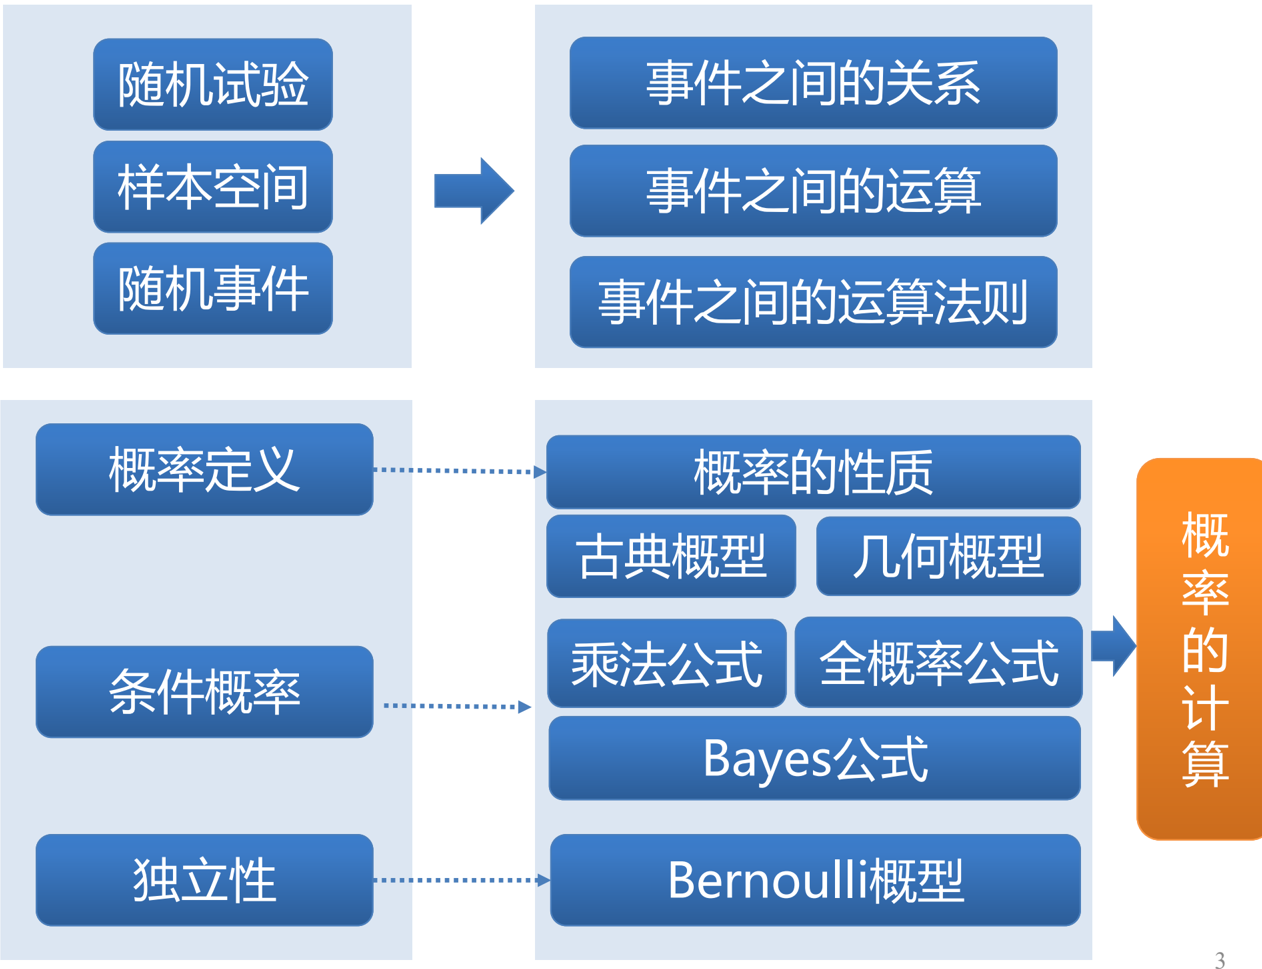
\includegraphics[width=0.7\textwidth]{figures/fig_knowledge_structure.png}
    \caption{知识结构图}
    \label{fig:knowledge_structure}
\end{figure}

\subsection{基本概念}

\textbf{实验 v.s. 试验}（《现代汉语词典》定义）
\begin{itemize}[leftmargin=2em]
    \item \textbf{实验}：为了检验某种科学理论或假设而进行某种操作或从事某种活动。
    \item \textbf{试验}：为了察看某事的结果或某物的性能而从事某种活动。
\end{itemize}

\textbf{随机试验}$E$是满足如下三个特征的试验：
\begin{enumerate}[label=\arabic*.,leftmargin=2em]
    \item \textbf{可重复性}：可在相同条件下重复进行；
    \item \textbf{不确定性}：一次试验之前无法确定具体出现哪种结果；
    \item \textbf{完备性}：能确定所有的可能结果。
\end{enumerate}

\textbf{随机试验}$\to$\textbf{随机事件}$\to$\textbf{概率}

\begin{itemize}[leftmargin=2em]
    \item \textbf{样本点}：随机试验的单个结果。
    \item \textbf{样本空间}$S$：随机试验所有可能的结果组成的集合。
    \item \textbf{随机事件}：样本空间的任意一个子集。
    \item \textbf{基本事件}：有一个样本点组成的单点集。
    \item \textbf{必然事件}$S$：样本空间中所有样本点构成的集合。
    \item \textbf{不可能事件}$\varnothing$：不包含任何样本点的空集。
\end{itemize}

\begin{remark}
\begin{enumerate}[label=\arabic*.,leftmargin=2em]
    \item 随机事件是定义在随机试验基础上的；概率是随机事件的概率。
    \item 随机事件的"集合"定义形式，促成了事件的运算与集合运算的关系。
\end{enumerate}
\end{remark}

\subsection{事件之间的关系和运算}

\begin{table}[htbp]
\centering
\caption{事件之间的关系和运算}
\begin{tabular}{@{}ccccc@{}}
\toprule
\textbf{关系/运算} & \textbf{符号表示} & \textbf{概率论} & \textbf{集合论}\\
\midrule
包含关系 & $A\subset B$ & 事件$A$发生必有事件$B$发生 & $A$是$B$的子集\\
等价关系 & $A=B$ & 若$A\subset B$且$B\subset A$，则事件$A$与事件$B$相等 & $A$与$B$相等\\
和事件 & $A\cup B$ & 事件$A$与$B$至少有一个发生 & $A$与$B$的并集\\
积事件 & $A\cap B\doteq AB$ & 事件$A$与$B$同时发生 & $A$与$B$的交集\\
互不相容 & $A\cap B=\varnothing$ & 事件$A$与$B$不能同时发生 & $A$与$B$无交集\\
对立事件（逆事件） & $A\cap B=\varnothing$且$A\cup B=S$，则$B\doteq\bar{A}$ & 对每次试验而言，事件$A$、$B$有且仅有一个发生 & $A$与$B$互补\\
\bottomrule
\end{tabular}
\end{table}

\subsection{事件之间的运算规则}

\begin{itemize}[leftmargin=2em]
    \item \textbf{交换律}：$A\cup B=B\cup A$，$A\cap B=B\cap A$
    \item \textbf{结合律}：
    \[
    A\cup(B\cup C)=(A\cup B)\cup C,\quad A\cap(B\cap C)=(A\cap B)\cap C
    \]
    \item \textbf{分配律}：
    \[
    A\cup(B\cap C)=(A\cup B)\cap(A\cup C),\quad A\cap(B\cup C)=(A\cap B)\cup(A\cap C)
    \]
    \item \textbf{De Morgan律}：
    \[
    \overline{A\cup B}=\bar{A}\cap\bar{B},\quad \overline{A\cap B}=\bar{A}\cup\bar{B}
    \]
\end{itemize}

\begin{example}[事件运算实例]
\begin{itemize}[leftmargin=2em]
    \item "$A,B,C$中至少有一个发生"：$A\cup B\cup C$
    \item "$A,B,C$中至少有两个发生"：$AB\cup BC\cup AC$
    \item "$A,B,C$中最多有一发生"：
    \[
    A\bar{B}\bar{C}+\bar{A}B\bar{C}+\bar{A}\bar{B}C+\bar{A}\bar{B}\bar{C}=\overline{AB\cup BC\cup AC}
    \]
\end{itemize}
\end{example}

\begin{example}[De Morgan律证明]
证明$\overline{A\cup B}=\bar{A}\cap\bar{B}$。

\textbf{解}：
\[
\begin{aligned}
\forall x\in\overline{A\cup B}&\Rightarrow x\not\in A\cup B\\
&\Rightarrow x\not\in A\text{ 且 }x\not\in B\\
&\Rightarrow x\in\bar{A}\text{ 且 }x\in\bar{B}\\
&\Rightarrow x\in\bar{A}\cap\bar{B}\\
&\Rightarrow\overline{A\cup B}\subseteq\bar{A}\cap\bar{B}.
\end{aligned}
\]
\[
\begin{aligned}
\forall x\in\bar{A}\cap\bar{B}&\Rightarrow x\in\bar{A}\text{ 且 }x\in\bar{B}\\
&\Rightarrow x\not\in A\text{ 且 }x\not\in B\\
&\Rightarrow x\not\in A\cup B\\
&\Rightarrow x\in\overline{A\cup B}\\
&\Rightarrow\bar{A}\cap\bar{B}\subseteq\overline{A\cup B}.
\end{aligned}
\]
\end{example}

\section{频率与概率}

\textbf{频率}：描述事件发生的频繁程度。

\textbf{概率}：表征随机事件在一次试验中发生的可能性大小。

\subsection{频率与概率的定义}

事件$A$发生的\textbf{频率}记为$f_n(A)=\dfrac{n_A}{n}$：
\begin{enumerate}[label=\arabic*.,leftmargin=2em]
    \item $0\leq f_n(A)\leq1$
    \item $f_n(\Omega)=1$
    \item 若$A_1,A_2,\ldots,A_k$两两互不相容事件，则
    \[
    f_n(A_1\cup A_2\cup\cdots\cup A_k)=f_n(A_1)+f_n(A_2)+\cdots+f_n(A_k)
    \]
\end{enumerate}

事件$A$发生的\textbf{概率}记为$P(A)$：
\begin{enumerate}[label=\arabic*.,leftmargin=2em]
    \item $P(A)\geq0$；非负性
    \item $P(\Omega)=1$；规范性
    \item 若$A_1,A_2,\ldots$两两互不相容事件，即$A_iA_j=\varnothing$，$i\neq j$，$i,j=1,2,\ldots$，则
    \[
    P(A_1\cup A_2\cup\cdots)=P(A_1)+P(A_2)+\cdots\quad\text{（可列可加性）}
    \]
\end{enumerate}

\textbf{频率的稳定性}：$n\to\infty$，$f_n(A)\to P(A)$。

\subsection{概率的性质与推广}

\textbf{性质1}：$P(\varnothing)=0$

\textbf{性质2}：$P(A)\leq1$

\textbf{性质3}：若$A_1,A_2,\ldots,A_n$是两两不相容事件，则
\[
P(A_1\cup A_2\cup\cdots\cup A_n)=P(A_1)+P(A_2)+\cdots+P(A_n)\quad\text{（有限可加性）}
\]

\textbf{性质4}（包含可减性）：$A\subset B\Rightarrow P(B-A)=P(B)-P(A)$

\textbf{性质5}（逆事件的概率公式）：$P(\bar{A})=1-P(A)$

\textbf{性质6}：$P(A\cup B)=P(A)+P(B)-P(AB)$

\textbf{一般推广}：
\[
P(B\bar{A})=P(B-A)=P(B)-P(AB)
\]
\[
P(\bar{A}\bar{B}\bar{C})=P(\overline{A\cup B\cup C})=1-P(A\cup B\cup C)
\]

\textbf{加法公式推广}：
\[
P(A_1\cup A_2\cup\cdots\cup A_n)=\sum_{i=1}^{n}P(A_i)-\sum_{1\leq i<j\leq n}P(A_iA_j)+\sum_{1\leq i<j<k\leq n}P(A_iA_jA_k)+\cdots+(-1)^{n-1}P(A_1A_2\ldots A_n)
\]

\begin{example}[加法公式证明]
证明$P(A\cup B\cup C)=P(A)+P(B)+P(C)-P(AB)-P(AC)-P(BC)+P(ABC)$。

\textbf{解}：
\[
A\cup B\cup C=A\cup(B-AB)\cup(C-C(A\cup B))
\]
因为$A$、$B-AB$、$C-C(A\cup B)$两两互斥，所以
\[
\begin{aligned}
P(A\cup B\cup C)&=P(A)+P(B-AB)+P(C-C(A\cup B))\\
&=P(A)+P(B)-P(AB)+P(C)-P(C(A\cup B))\\
&=P(A)+P(B)-P(AB)+P(C)-P(AC\cup BC)\\
&=P(A)+P(B)-P(AB)+P(C)-P(AC)-P(BC)+P(ABC)\\
&=P(A)+P(B)+P(C)-P(AB)-P(AC)-P(BC)+P(ABC).
\end{aligned}
\]
\end{example}

\section{古典概型与几何概型}

\subsection{古典概型（等可能概型）}

\textbf{特点}：
\begin{enumerate}[label=\arabic*.,leftmargin=2em]
    \item 样本空间的元素只有有限个；（有限性）
    \item 每个基本事件发生的可能性相同。（等可能性）
\end{enumerate}

\textbf{随机事件的概率}：
\[
P(A)=\frac{A\text{ 中元素个数}}{\Omega\text{ 中元素个数}}=\frac{N(A)}{N(\Omega)}
\]

\textbf{几个经典问题}：
\begin{enumerate}[label=\arabic*.,leftmargin=2em]
    \item \textbf{无放回抽样}：超几何分布，$p_k=\dfrac{C_D^kC_{N-D}^{n-k}}{C_N^n}$
    \item \textbf{有放回抽样}：二项分布，$p_k=\dfrac{C_n^kD^k(N-D)^{n-k}}{N^n}$
    \item \textbf{生日问题}：$n$个人生日各不相同，$p=\dfrac{365!}{365^n(365-n)!}$
    \item \textbf{分组数量}：$n$个球分$m$组，第$i$组有$n_i$个球，一共有$\dfrac{n!}{n_1!n_2!\cdots n_m!}$种分法
    \item \textbf{有放回与无放回抽签}：$\dfrac{a}{a+b}$
\end{enumerate}

\subsection{几何概型}

古典概型只考虑了有限等可能的随机试验，几何概型考虑了有无穷多个等可能结果的随机试验。

\textbf{几何概型的随机试验特点}：
\begin{enumerate}[label=\arabic*.,leftmargin=2em]
    \item 样本空间$\Omega$是一个几何区域；
    \item 随机试验$E$相当于在区域内任意地取点，且取到每一点都是等可能的。
\end{enumerate}

如果试验$E$是向区域内任意取点，事件$A$对应于点落在$\Omega$内的某区域$A$，则
\[
P(A)=\frac{m_A}{m_\Omega}
\]
其中，$m_\Omega$、$m_A$是可度量区域$\Omega$、$A$的度量（如线段长度、平面区域面积、空间区域的体积等）。

\begin{example}[会面问题]
甲、乙二人约定在5点到12点之间在某地会面，先到者等一个小时后即离去。设二人在这段时间内的各时刻到达是等可能的，且二人互不影响。求二人能会面的概率。

\begin{figure}[htbp]
    \centering
    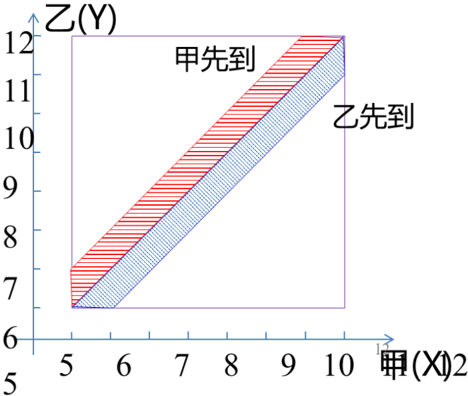
\includegraphics[width=0.5\textwidth]{figures/fig_meeting_region.png}
    \caption{正方形区域 $[5,12]\times[5,12]$，阴影区域为 $|x-y|\leq1$ 的带状区域}
    \label{fig:meeting_region}
\end{figure}
\end{example}

\section{条件概率与Bayes公式}

\subsection{条件概率}

\textbf{条件概率}：在事件$A$发生的条件下事件$B$发生的概率。

\textbf{公式法}：
\[
P(B\mid A)=\frac{P(AB)}{P(A)},\quad\text{其中 }P(A)>0
\]

\textbf{缩小样本空间法}——适用于古典概型

设事件$A$所含样本点数为$n_A$，事件$AB$所含样本点数为$n_{AB}$，则
\[
P(B\mid A)=\frac{n_{AB}}{n_A}
\]

\begin{remark}
条件概率与无条件概率的大小无确定关系，$P(B)$与$P(B\mid A)$无确定的大小关系。
\end{remark}

\subsection{乘法公式和全概率公式}

\textbf{乘法公式}：
\[
P(AB)=P(B\mid A)P(A),\quad P(A)>0
\]

$n$个事件：假设$P(A_1A_2\ldots A_{n-1})>0$，有：
\[
P(A_1A_2\ldots A_n)=P(A_n\mid A_1A_2\ldots A_{n-1})\cdot P(A_{n-1}\mid A_1A_2\ldots A_{n-2})\cdots P(A_2\mid A_1)P(A_1)
\]

\textbf{全概率公式}

\textbf{划分}："交为空，并为全"

$B_1,B_2,\ldots,B_n$是样本空间$\Omega$的一个划分
\[
P(A)=\sum_{i=1}^{n}P(AB_i)=\sum_{i=1}^{n}P(B_i)P(A\mid B_i)
\]
（已知原因/因素，求结果）

\subsection{Bayes公式}

\begin{figure}[htbp]
    \centering
    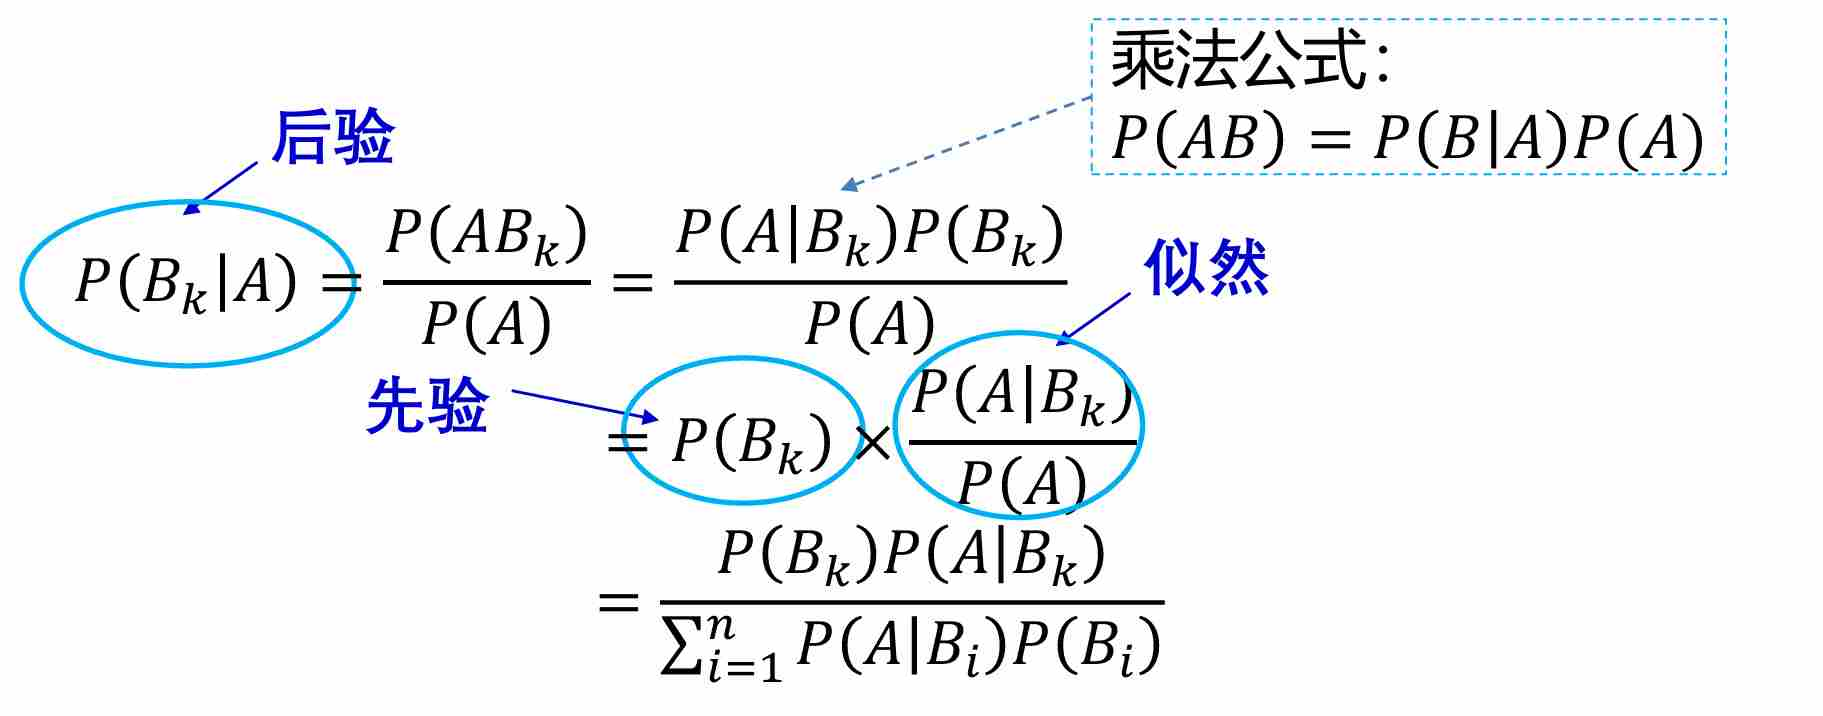
\includegraphics[width=0.5\textwidth]{figures/fig_bayes_diagram.jpg}
    \caption{Bayes公式示意图（先验、似然、后验的关系）}
    \label{fig:bayes_diagram}
\end{figure}

\[
P(B_k\mid A)=\frac{P(AB_k)}{P(A)}=\frac{P(A\mid B_k)P(B_k)}{P(A)}=\frac{P(B_k)P(A\mid B_k)}{\sum_{i=1}^{n}P(A\mid B_i)P(B_i)}
\]

\textbf{理解1}：【执果溯因】已知结果，求原因的可能性。

\textbf{理解2}：【经验更新】先验概率，结合新获得的信息，得到修正后的结论。

\begin{example}[拼写检查]
背景材料：一本字典$D$，一个语料库$S$。

问题：用户输入了一个单词$w$，判断此单词是否正确（即是否可在字典$D$中查询到），如果$w$不正确，给出可能的正确单词拼写。

如果$w$不在字典$D$中，则$w$拼写错误。

为了找出最可能正确的单词，考察字典中与$w$形近的单词$c$：

$P(c)$：单词$c$出现的先验概率，可从语料库$S$中统计$c$出现的频率。

通过Bayes公式利用似然函数$P(w\mid c)$更新概率：
\[
P(c\mid w)=\frac{P(w\mid c)P(c)}{P(w)}\propto P(w\mid c)P(c)
\]

$P(w\mid c)$：在试图拼写$c$的情况下，出现拼写错误$w$的概率。可根据$w$与$c$的距离计算：
\begin{itemize}[leftmargin=2em]
    \item 莱文斯坦距离（Levenshtein distance）
    \item 最长公共子串长度
\end{itemize}
\end{example}

\section{独立性}

\subsection{两事件独立的定义}

\[
P(AB)=P(A)P(B)
\]

\subsection{两事件独立性的性质}

\begin{itemize}[leftmargin=2em]
    \item $P(A)>0$，事件$A$与$B$相互独立的充分必要条件：$P(B\mid A)=P(B)$
    \item \textbf{逆事件的独立性}：若随机事件$A$与$B$相互独立，则$\bar{A}$与$B$，$A$与$\bar{B}$，$\bar{A}$与$\bar{B}$也相互独立
    \item 必然事件$S$与任意随机事件$A$相互独立
    \item 不可能事件$\varnothing$与任意随机事件$A$相互独立
\end{itemize}

\begin{remark}
\begin{enumerate}[label=\arabic*.,leftmargin=2em]
    \item \textbf{两事件相互独立 vs 互不相容}
    \begin{itemize}
        \item "$A$与$B$互不相容"指两事件不能同时发生，即$AB=\varnothing$。（$P(AB)=0\nRightarrow AB$互不相容）
        \item "$A$与$B$相互独立"指$A$是否发生不影响$B$发生的概率
    \end{itemize}
    \item 设事件$A$与$B$满足$P(A)P(B)\neq0$，则互不相容与相互独立不能同时成立，即
    \begin{itemize}
        \item 若事件$A$与$B$相互独立，则$AB\neq\varnothing$
        \item 若$AB=\varnothing$，则事件$A$与$B$不相互独立
    \end{itemize}
    \item 区分"对立事件"与"相互独立事件"：对立事件不相互独立。
\end{enumerate}
\end{remark}

\subsection{三个事件的独立性}

设$A$、$B$、$C$是三个随机事件，如果
\[
\begin{cases}
P(AB)=P(A)P(B)\\
P(AC)=P(A)P(C)\\
P(BC)=P(B)P(C)\\
P(ABC)=P(A)P(B)P(C)
\end{cases}
\]
四个等式缺一不可，则称$A$、$B$、$C$是相互独立的随机事件。

\begin{remark}
\begin{enumerate}[label=\arabic*.,leftmargin=2em]
    \item 在三个事件独立性的定义中，四个等式缺一不可。即前三个等式的成立不能推出第四等式的成立；反之，最后一个等式的成立也推不出前三个等式的成立。
    \item 若$A,B,C$是相互独立的三个事件，则通过事件$B$、$C$运算得到的事件也与事件$A$相互独立，例如$(A,\overline{B\cup C})$，$(A,\overline{BC})$，$(A,\overline{B}-\overline{C})$，$(A,\overline{B\cup C})$，$(A,\overline{BC})$，$(A,\bar{B}\bar{C})$等。
\end{enumerate}
\end{remark}

\subsection{$n$个事件的相互独立性}

设$A_1,A_2,\ldots,A_n$为$n$个随机事件，若下列等式成立
\[
\begin{cases}
P(A_iA_j)=P(A_i)P(A_j) & (1\leq i<j\leq n)\\
P(A_iA_jA_k)=P(A_i)P(A_j)P(A_k) & (1\leq i<j<k\leq n)\\
\cdots\cdots & \cdots\\
P(A_1A_2\ldots A_n)=P(A_1)P(A_2)\cdots P(A_n)
\end{cases}
\]
则称$A_1,A_2,\ldots,A_n$这$n$个随机事件相互独立。

\section{Bernoulli概型}

\textbf{Bernoulli试验}：若随机试验$E$只有两个结果。一般地，我们将这两个结果记为$A$与$\bar{A}$，分别称为"成功"与"失败"。

\textbf{$n$重Bernoulli试验}：独立重复地进行$n$次Bernoulli试验
\begin{itemize}[leftmargin=2em]
    \item "重复"：指每次试验中$A$发生的概率（即"成功"的概率）不变
    \item "独立"：指各次试验的结果相互独立
\end{itemize}

\textbf{$n$重Bernoulli试验中恰好成功$k$次的概率}：

设在一次Bernoulli试验中，$P(A)=p$，$P(\bar{A})=1-p=q$。

事件$B_{n,k}=\{n\text{ 重Bernoulli试验中事件}A\text{ 恰好发生}k\text{ 次}\}$的概率：
\[
P(B_{n,k})=C_n^kp^k(1-p)^{n-k},\quad k=0,1,2,\ldots,n
\]

\section{核心内容总结}

\begin{enumerate}[label=\arabic*.,leftmargin=2em]
    \item \textbf{随机事件及其概率}
    \begin{itemize}
        \item 随机事件、样本点、样本空间
        \item 事件关系及运算 $\nabla$ 集合关系及运算
        \item 事件的集合形式表达
    \end{itemize}
    \item \textbf{频率与概率}
    \begin{itemize}
        \item 概率定义的三要素
        \item 概率的性质：可列可加性\&有限可加性（互不相容）；包含可减性；加法公式（两个事件、多个事件）
    \end{itemize}
    \item \textbf{古典概型与几何概型}
    \begin{itemize}
        \item 定义条件：古典概型（每种结果等可能，且所有结果数有限）；几何概型（每种结果等可能，且所有结果数无限）
        \item 计算方式：古典概型（取法比值，$N(A)/N(\Omega)$）；几何概型（度量比值，$m_A/m_\Omega$）
    \end{itemize}
    \item \textbf{条件概率与Bayes公式}
    \begin{itemize}
        \item 条件概率：公式法、缩小样本空间法
        \item 乘法公式：$P(AB)=P(B\mid A)P(A)$
        \item 全概率公式：$P(A)=\sum_{i=1}^{n}P(B_i)P(A\mid B_i)$
        \item Bayes公式：$P(B_k\mid A)=\dfrac{P(B_k)P(A\mid B_k)}{\sum_{i=1}^{n}P(A\mid B_i)P(B_i)}$
    \end{itemize}
    \item \textbf{独立性}
    \begin{itemize}
        \item 定义；独立 $\nabla$ 互不相容
        \item 3个事件的相互独立；$n\geq3$个事件的相互独立
    \end{itemize}
    \item \textbf{Bernoulli概型}
    \begin{itemize}
        \item Bernoulli试验；$n$重Bernoulli试验
        \item $n$重Bernoulli试验中恰好成功$k$次的概率
    \end{itemize}
\end{enumerate}

\section{作业题情况}

\begin{example}[《概率论及其应用》1.8 \#14]
证明$\overline{A\cup B}=\bar{A}\cap\bar{B}$。

多种证明方式：根据定义，画图，利用公式等。本题的目的是考察对定义的了解，所以推荐使用定义证明。

\textbf{解}：
\[
\begin{aligned}
\forall x\in\overline{A\cup B}&\Rightarrow x\not\in A\cup B\\
&\Rightarrow x\not\in A\text{ 且 }x\not\in B\\
&\Rightarrow x\in\bar{A}\text{ 且 }x\in\bar{B}\\
&\Rightarrow x\in\bar{A}\cap\bar{B}\\
&\Rightarrow\overline{A\cup B}\subseteq\bar{A}\cap\bar{B}.
\end{aligned}
\]
\[
\begin{aligned}
\forall x\in\bar{A}\cap\bar{B}&\Rightarrow x\in\bar{A}\text{ 且 }x\in\bar{B}\\
&\Rightarrow x\not\in A\text{ 且 }x\not\in B\\
&\Rightarrow x\not\in A\cup B\\
&\Rightarrow x\in\overline{A\cup B}\\
&\Rightarrow\bar{A}\cap\bar{B}\subseteq\overline{A\cup B}.
\end{aligned}
\]
\end{example}

\begin{example}[《概率论及其应用》1.8 \#16(b)]
$ABC=AB(C\cup B)$不总是成立，除非$AB\subset C$。

$A\bar{B}C\subset A\cup B$
\end{example}

\begin{example}[《概率论及其应用》2.10 \#9]
计算：$n$个球随机放入$n$个盒，恰有一盒空着的概率。

\textbf{解}：
\begin{itemize}[leftmargin=2em]
    \item 总的放法个数：$n^n$
    \item 空盒的可能个数：$C_n^1$
    \item 问题变为：$n$个球装入$n-1$个盒子，不能有空
    \item 从而某个盒子必须有2个球，两个球的构成方式：$C_n^2$
    \item 放入盒子的方式：$(n-1)!$
    \item 结果为：
    \[
    \frac{C_n^1\cdot C_n^2\cdot(n-1)!}{n^n}=\frac{C_n^2\cdot n!}{n^n}
    \]
\end{itemize}
\end{example}

\begin{example}[《概率论及其应用》2.10 \#21]
谣言的传播：在一个拥有$n+1$个居民的城市里，某人告诉第二个人一个谣言，第二个人又把谣言告诉第三个人，如此等等。在每一步中，谣言的接收者都是随机地从$n$个居民中挑选。

求下述两事件的概率：谣言传播$r$次后，
\begin{enumerate}[label=(\alph*)]
    \item 还没有回到第一个造谣者；
    \item 没有一个人两次听到谣言。
\end{enumerate}

当每一次都把谣言同时告诉由城市中随机选取的$N$个居民时，(a)(b)两事件的概率等于多少？

\textbf{解}：$N=1$时，共有$n^r$种等可能传播情况
\begin{enumerate}[label=(\alph*)]
    \item 还没有回到第一个造谣者的情况有$n(n-1)^{r-1}$种
    \[
    P_A=\frac{n(n-1)^{r-1}}{n^r}=\left(1-\frac{1}{n}\right)^{r-1}
    \]
    \item 没有一人两次听到谣言的情况有$A_n^r=\dfrac{n!}{(n-r)!}$种
    \[
    P_B=\frac{A_n^r}{n^r}
    \]
\end{enumerate}

\textbf{解（续）}：若每次传播随机选取$N$个居民，共有$(C_n^N)^r$种等可能情况
\begin{enumerate}[label=(\alph*)]
    \item 没有回到第一个造谣者的情况有$C_n^N(C_{n-1}^N)^{r-1}$种
    \[
    P_A=\frac{C_n^N(C_{n-1}^N)^{r-1}}{(C_n^N)^r}=\left(1-\frac{N}{n}\right)^{r-1}
    \]
    \item 没有一人两次听到谣言的情况有$C_n^NC_{n-N}^NC_{n-2N}^N\cdots C_{n-(r-1)N}^N$种
    \[
    P_B=\frac{C_n^NC_{n-N}^NC_{n-2N}^N\cdots C_{n-(r-1)N}^N}{(C_n^N)^r}=\frac{n!}{(N!)^r(n-rN)!}
    \]
\end{enumerate}
\end{example}

\begin{example}[《概率论及其应用》2.10 \#24(b)]
求6个人的生日恰巧在两个月中的概率。（假定任何一个人生于12个月中之任一月都是等概率的）

\textbf{解}：
\[
\frac{C_{12}^2(2^6-2)}{12^6}
\]
本题结果中分子的乘子容易写成$2^6$而忘记减2，2表示6个人全部在其中的一个月生日的事件数。
\end{example}

\begin{example}[《概率论及其应用》2.10 \#38]
印刷错误：假设书中每一页都有$N$个印刷符号，他们有可能印错。全书共有$n=500$页，$r=50$个印错符号。证明：
\begin{enumerate}[label=(\alph*)]
    \item 第$1,2,\ldots,n$页分别含有$r_1,r_2,\ldots,r_n$个印错符号的概率为
    \[
    \frac{C_N^{r_1}C_N^{r_2}\cdots C_N^{r_n}}{C_{nN}^r}
    \]
    \item 当$N$充分大后，
    \[
    \frac{C_N^{r_1}C_N^{r_2}\cdots C_N^{r_n}}{C_{nN}^r}
    \]
    逼近$\dfrac{r!}{r_1!r_2!\cdots r_n!n^r}$。$r$个错误分布在$n$页的问题近似于$r$个球随机放入$n$个盒子的问题。
\end{enumerate}

\textbf{提示}：$N\to+\infty$，$N\gg c\Longrightarrow\dfrac{N!}{(N-c)!}\sim N^c$
\end{example}

\begin{example}[《概率论与数理统计》1.8（2）]
求至少有2件次品的概率。

\textbf{解}：
\[
P(X\geq2)=1-P(0)-P(1)
\]
\end{example}

\begin{example}[《概率论与数理统计》1.12]
50只铆钉随机地取来用在10个部件上，其中有3只铆钉强度太弱。每个部件用3只铆钉。若将3只强度太弱的铆钉都钉在一个部件上，则这个部件强度就太弱。问发生一个部件强度太弱的概率是多少？

\textbf{解法1}：

50只铆钉随机用在10个部件上的可能情况：$\dfrac{A_{50}^{30}}{(3!)^{10}}$

一个部件强度为弱的可能情况：$C_{10}^1\dfrac{A_{47}^{27}}{(3!)^9}$

发生一个部件强度太弱的概率：
\[
P=\frac{C_{10}^1\dfrac{A_{47}^{27}}{(3!)^9}}{\dfrac{A_{50}^{30}}{(3!)^{10}}}=\frac{1}{1960}
\]

\textbf{解法2}：令$A_i$表示事件"第$i$号部件强度太弱"

从50只铆钉中取出3只放在第$i$号部件上的可能取法：$C_{50}^3$

强度太弱的铆钉都装在第$i$号部件上的可能取法：$C_3^3=1$

\[
P(A_i)=\frac{1}{C_{50}^3}=\frac{1}{19600}
\]

由于$A_1,A_2,\ldots,A_{10}$两两互不相容，
\[
P(A_1\cup A_2\cup\cdots\cup A_{10})=P(A_1)+P(A_2)+\cdots+P(A_{10})=\frac{1}{1960}
\]
\end{example}

\section{典型例题}

\begin{example}[例1]
已知$A$、$B$、$C$是三个两两独立的事件，且$ABC=\varnothing$，$P(A\cup B\cup C)=\dfrac{9}{16}$，$P(A)=P(B)=P(C)$，求$P(A)$。

\textbf{解}：
\[
\begin{aligned}
\frac{9}{16}&=P(A\cup B\cup C)\\
&=P(A)+P(B)+P(C)-P(AB)-P(AC)-P(BC)+P(ABC)\\
&=3P(A)-3P(A)^2
\end{aligned}
\]
求解得$P(A)=\dfrac{3}{4}$或$P(A)=\dfrac{1}{4}$。

又因为$P(A)<P(A\cup B\cup C)=\dfrac{9}{16}$，故$P(A)=\dfrac{1}{4}$。
\end{example}

\begin{example}[例2]
$A$、$B$是两个随机事件，$P(A\cup B)=0.7$，$P(A)=0.4$。
\begin{enumerate}[label=(\arabic*)]
    \item 若$A,B$互不相容，求$P(B)$；
    \item 若$A,B$相互独立，求$P(B)$；
    \item 若$P(B\mid A)=0.6$，求$P(B)$。
\end{enumerate}

\textbf{解}：$P(A\cup B)=P(A)+P(B)-P(AB)$

(1) $P(A\cup B)=P(A)+P(B)=0.7$，$P(B)=0.7-0.4=0.3$

(2) $P(AB)=P(A)P(B)$
\[
P(B)=\frac{P(A\cup B)-P(A)}{P(\bar{A})}=\frac{0.7-0.4}{0.6}=0.5
\]

(3) $P(AB)=P(A)P(B\mid A)$
\[
P(B)=P(A\cup B)-P(A)+P(A)P(B\mid A)=0.7-0.4+0.4\times0.6=0.5
\]
\end{example}

\begin{example}[例3]
在长为1的线段上任取两点，分成3个线段，求这些线段能构成三角形的概率。

\textbf{解}：设取的三个线段长度分别为$x,y,1-x-y$。$x,y$取值满足$x+y<1,x>0,y>0$，即落在下图三角形$AOB$中。

若三个线段要构成三角形，则需满足任意两边之和大于第三边，即满足：
\[
\begin{cases}
1-x-y<x+y<1\\
y<x+(1-x-y)<1\\
x<y+(1-x-y)<1
\end{cases}
\Rightarrow
\begin{cases}
x+y>0.5\\
y<0.5\\
x<0.5
\end{cases}
\]
即落在图中阴影区域内。
\begin{figure}[htbp]
    \centering
    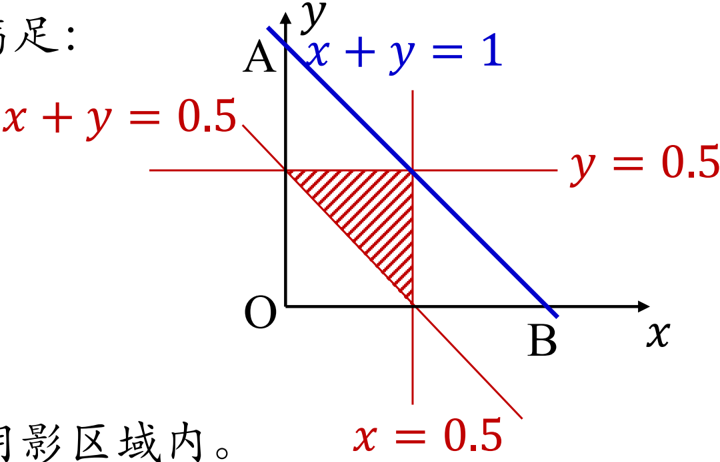
\includegraphics[width=0.5\textwidth]{figures/fig_triangle_AOB.png}
    \caption{三角形 $AOB$，$x+y=1$ 为斜边，阴影区域为形成三角形的条件}
    \label{fig:triangle_AOB}
\end{figure}

所以，这些线段能构成三角形的概率为$0.25$。
\end{example}

\begin{example}[例4]
从混有5张假钞的20张百元钞票中任意抽出2张，将其中1张放到验钞机上检验发现是假钞。求2张都是假钞的概率。

\textbf{解}：令事件$A$表示抽到2张都是假钞，事件$B$表示2张中至少有1张假钞。

则所求概率是$P(A\mid B)$（而不是$P(A)$！）

\[
P(A\mid B)=\frac{P(AB)}{P(B)}=\frac{P(A)}{P(B)}=\frac{C_5^2/C_{20}^2}{(C_5^2+C_5^1C_{15}^1)/C_{20}^2}=\frac{C_5^2}{C_5^2+C_5^1C_{15}^1}=\frac{10}{85}=0.118
\]
\end{example}

\begin{example}[例5]
对以往的数据分析结果表明当机器调整得良好时，产品的合格率为90\%，而当机器发生某一故障时，其合格率为30\%。每天早上机器开动时，机器调整良好的概率为75\%。已知某天早上第一件产品是合格品，试求机器调整得良好的概率是多少？

\textbf{解}：设事件$A$：产品合格；事件$B$：机器调整良好，且$P(A\mid B)=0.9$；事件$\bar{B}$：机器发生故障，且$P(A\mid\bar{B})=0.3$。

\[
P(B\mid A)=\frac{P(A\mid B)P(B)}{P(A\mid B)P(B)+P(A\mid\bar{B})P(\bar{B})}=\frac{0.9\times0.75}{0.9\times0.75+0.3\times0.25}=0.9
\]
\end{example}

\end{document}